% IEEE standard conference template; to be used with:
%   spconf.sty  - LaTeX style file, and
%   IEEEbib.bst - IEEE bibliography style file.
% --------------------------------------------------------------------------

\documentclass[letterpaper]{article}
\usepackage{spconf,amsmath,amssymb,graphicx}
\usepackage{todonotes}
\usepackage{hyperref}
\usepackage[ruled]{algorithm2e}
\usepackage{seqsplit}

% Example definitions.
% --------------------
% nice symbols for real and complex numbers
\newcommand{\R}[0]{\mathbb{R}}
\newcommand{\C}[0]{\mathbb{C}}

% bold paragraph titles
\newcommand{\mypar}[1]{{\bf #1.}}

% add page number to bottom
\pagestyle{plain}


% Title.
% ------
\title{Parallelizing Myers' algorithm for the longest common subsequence problem}

\name{Josua Cantieni, Lowis Engel, Pascal Maillard, Philippe Voinov} 
\address{Department of Computer Science\\ ETH Z\"urich\\Z\"urich, Switzerland}


\begin{document}
%\ninept
%
\maketitle
%

%The hard page limit is 6 pages in this style. Do not reduce font size
%or use other tricks to squeeze. This pdf is formatted in the American letter format, so the spacing may look a bit strange when printed out.


\begin{abstract}
%Describe in concise words what you do, why you do it (not necessarily
%in this order), and the main result.  The abstract has to be
%self-contained and readable for a person in the general area. You
%should write the abstract last.
The longest common subsequence is the longest possible subsequence of symbols that two input sequences have in common. Its most common applications are in finding the smallest number of differences in text files (usually source code) or aligning common regions of DNA strands.

In this report, we present our approach to parallelizing Myers' sequential algorithm. We implemented two different versions: statically distributing each DP table row across MPI workers and a priority approach that avoids idle waiting by dynamically prioritizing entries needed by other workers. We applied vectorization to further improve the performance.

We analyze the performance using both synthetic randomly generated input sequences and real DNA (nucleic acid) sequences. Overall, our row-wise implementation scales nearly linearly with the amount of workers and does not suffer from any additional overhead, as long as that the inputs are sufficiently large.
\end{abstract}
\section{Introduction}\label{sec:intro}

\mypar{Motivation} The longest common subsequence (LCS) problem is the problem of finding the longest (not necessarily contiguous) subsequence that is shared by two input strings. This problem occurs very widely in practice. For example, the two sequences $ABCD$ and $ACBAD$ have the longest common subsequences $ACD$ and $ABD$. The length of the LCS is unique, although multiple subsequences with that length might exist.

LCS algorithms are at the core of comparison tools like ``diff'', which are ubiquitous when working with source code. These comparisons are also used extensively in version control systems. Outside of the software domain, the longest common subsequence problem is extremely important in biology - LCS is the exact solution to DNA nucleotide \emph{sequence alignment}. However, it is important to note that heuristic methods (BLAST \cite{altschul_basic_1990}) are often used today, since they allow fast search of very large databases of genetic sequences.

There exist various specialized LCS algorithms which achieve faster runtime or lower memory usage than general algorithms. One class of specialized algorithms provides improved runtime when both input sequences have significant similarities (edit distance not too large). This is generally the case when comparing two versions of a text document. For this reason algorithms of this class are nearly universally used by tools similar to ``diff''. However such algorithms are generally sequential.

We adapt the sequential LCS algorithm of Myers \cite{myers_anond_1986}, which is by far the most commonly used LCS algorithm for similar sequences, for parallel execution on a distributed memory system.

\mypar{Related work} Bergroth et al. prepared a survey \cite{bergroth_survey_2000} of various sequential LCS algorithms. They group the algorithms into three categories: ``row-by-row methods'', ``contour methods'' and ``diagonal methods''. The classic dynamic programming algorithm for LCS \cite{wagner_string--string_1974} is classified as a row-by-row method. Myers' algorithm \cite{myers_anond_1986} belongs to the class of diagonal methods. Diagonal methods are designed to be efficient when both input sequences are similar. 

Most parallel algorithms for the LCS problem are based on row-by-row sequential algorithms. Lu and Lin \cite{mi_lu_parallel_1994} presented a parallel algorithm of this class, achieving optimal complexity with a shared-memory machine model. Yang et al. \cite{jiaoyun_efficient_2010} designed a parallel LCS algorithm for GPUs (graphics processing units) by restructuring the classic DP (dynamic programming) table to reduce data dependencies.\linebreak These algorithms are fundamentally based on row-by-row methods, which are less efficient than diagonal methods for similar input sequences.

Allison and Dix \cite{allison_bit-string_1986} present a ``bit-parallel'' LCS algorithm (row-by-row method). Assuming a sufficiently small alphabet, their algorithm allows calculating multiple elements of the DP table in parallel, for example by using vector instructions. Their bit-parallel technique can be applied to other algorithms. We do not incorporate it into our algorithm, but do use vectorization within each DP cell.

Since Myers' algorithm \cite{myers_anond_1986} is an extremely popular LCS algorithm, we attempted to parallelize it. As far as we are aware, there are no published parallel versions of an LCS algorithm from the ``diagonal methods'' class, which Myers' algorithm belongs to. 
\section{Background}\label{sec:background}
We briefly explain the concept of edit distance and its relation to the longest common subsequence. We then present the sequential algorithm from Myers, which was the basis for our parallel implementation.

% Give a short, self-contained summary of necessary
% background information. For example, assume you present an
% implementation of sorting algorithms. You could organize into sorting
% definition, algorithms considered, and asymptotic runtime statements. The goal of the
% background section is to make the paper self-contained for an audience
% as large as possible. As in every section
% you start with a very brief overview of the section. Here it could be as follows: In this section 
% we formally define the sorting problem we consider and introduce the algorithms we use
% including a cost analysis.

% Explain the algorithm you use including their costs.
% As an aside, don't talk about "the complexity of the algorithm.'' It's incorrect, problems have a complexity, not algorithms.

% \mypar{Longest common subsequence}
% The longest common subsequence problem is the problem of finding the longest sequence that two input sequences have in common. A related problem is finding the longest common substring. However, in that case the solution sequence needs to appear consecutively within the input string.

\mypar{Edit distance}
The edit distance refers to the minimum number of changes required to transform one string into another. In the case where we only consider insertions and deletions, and exclude substitutions, the LCS problem is equivalent to finding the edit distance. All symbols that do not appear in the LCS count towards the edit distance.

To transform the first string into the second, we perform deletions for all symbols in the first sequence that are not part of the LCS and similarly insertions for the second sequence. Those changes are referred to as an edit script. % and the total number of changes is the edit distance.

%\mypar{Diff program} 
%In the context of computer science, it is a common problem to compare source files to different versions. In order to visualize changes better, a diff program can display the minimal number of changes by highlighting all symbols that are part of the edit script.

\mypar{Myers' algorithm}
Myers \cite{myers_anond_1986} takes a greedy approach to finding the solution in the edit graph of two sequences. It has an asymptotic runtime of $O(nd)$ where $n$ is the total length of the two sequences and $d$ is the size of the minimum edit script. This algorithm performs well when the sequences are similar and have a small $d$.

For constructing the edit graph, shown in figure \ref{edit_graph}, the two sequences A and B are placed along a grid. The solution for the shortest edit script can be constructed by finding the shortest path from $(0,0)$ to the bottom right corner. A horizontal or vertical segment represents an edit. A diagonal can only be taken if the two input sequences are identical.

\begin{figure}[hbt]\centering
  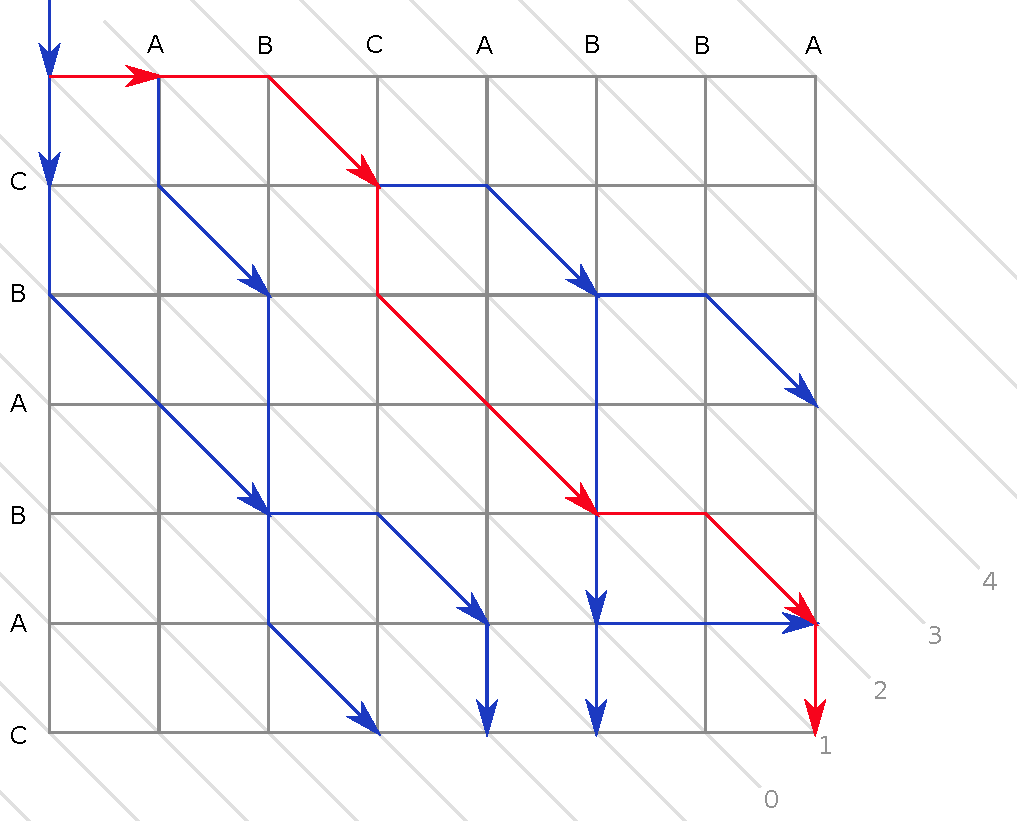
\includegraphics[width=0.9\linewidth]{images/edit-graph.pdf}
  \caption{Edit graph for comparison of two sequences \cite{edit_graph}. The solution for the shortest edit script is shown in red.
}
  \label{edit_graph}
\end{figure}

% Myers' algorithm pseudocode
\begin{algorithm}
\caption{Myers' LCS algorithm \cite{myers_anond_1986}}
\label{myers_algorithm}
\SetAlgoNoLine
\SetAlgoNoEnd
\DontPrintSemicolon
\scriptsize       % decrease font size

\KwSty{Constant} $MAX \in [0, M+N]$\;
$V:\ \KwSty{Integer}[-MAX\ ..\ MAX]$\;
\;
$V[1]\leftarrow 0$\;
\For{$d\leftarrow 0$ \KwTo $MAX$}{
    \For{$k\leftarrow -d$ \KwTo d in steps of 2}{
        \eIf{$k=-d$ or $k\ne d$ and $V[k-1]<V[k+1]$}{
            $x\leftarrow V[k+1]$\;
        }{
            $x\leftarrow V[k-1]+1$\;
        }
        $y\leftarrow x-k$\;
        \While{$x < N$ and $y < M$ and $a_{x+1} = b_{y+1}$}{$(x,y)\leftarrow (x+1,y+1)$\;}
        $V[k]\leftarrow x$\;
        \If{$x\ge N$ and $y \ge M$}{
            Length of shortest edit script is d\;
            \KwSty{STOP}\;
        }
    }
 }
\end{algorithm}

Myers' algorithm, shown in algorithm \ref{myers_algorithm}, goes through the diagonals shown in figure \ref{edit_graph} with an increasing edit distance and stores the coordinates of the furthest reachable point on each diagonal. The variables $N$ and $M$ represent the lengths of the sequences A and B.\\
To compute an entry on the diagonal $k$ and distance $d$, the previous paths can connect to it either by a horizontal or vertical move from its neighbors on the diagonals $k \pm 1$. Out of those two entries from the table for a distance of $d-1$, it takes the one with the higher x-value and follows the diagonal as long as the two sequences are identical. The new coordinates are then stored in the DP table.

The solution has been found once an entry reaches the coordinates $(N,M)$. The edit distance $d$ for that entry directly tells us the minimum edit distance. But the actual edit script has to be computed recursively.

\begin{figure}[hbt]\centering
  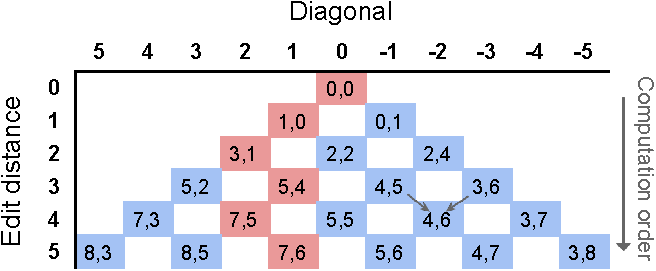
\includegraphics[width=0.95\linewidth]{images/dp_table.pdf}
  \caption{The DP table represents the furthest points on each diagonal that can be reached for a given edit distance. The arrows denote the dependencies of a single entry. The solution is marked in red and has an edit distance of 5.}
  \label{dp_table}
\end{figure}

Every entry depends on at most two entries from the previous row in the DP table (marked as arrows in figure \ref{dp_table}). If we only want the LCS length, it is not required to store the entire table, but only the previous row for the distance $d-1$. Thus the memory consumption is linear and no longer the limiting factor for very large input sequences. Myers presents an approach (``linear refinement'') to compute the solution recursively \cite{myers_anond_1986}. However, we will not go further into detail because it lies outside the scope of this report.
% Additionally, it is not necessary to store both coordinates. If we only store the x-coordinate for an entry, we can compute the intersection with the diagonal $k$ as $y = x - k$.

\section{Method}\label{sec:yourmethod}
We present our two different approaches to parallelize the algorithm and their major optimizations. Our implementations use MPI (``Message Passing Interface''). We also discuss a vectorization optimization that can be applied to both versions. Our source code and test cases are publicly available \cite{our_source}.


% Now comes the ``beef'' of the report, where you explain what you did. 
% Again, organize it in paragraphs with titles. As in every section
% you start with a very brief overview of the section.
% In this section, structure is very important so one can follow the technical content.
% Mention and cite any external resources that you used including libraries or other code.

\mypar{Row-wise algorithm}
The design of our algorithm is intentionally simple. We divide each row of our pyramid-shaped DP table into evenly spaced contiguous segments and assign exactly one to each worker. As the number of cells in each row is increased by one we increase the size of a segment by one. To ensure a balanced workload we increase each segment size in a round robin fashion.

Each worker calculates the cells in its segment from left to right. But in order to calculate the leftmost element the worker may depend on the rightmost element of the previous row from the left neighboring worker. Thus a worker has to wait for the neighboring worker to complete its segment in the previous row before the worker can start the next row. This can lead to an imbalance. In order to overcome this issue we prioritize the leftmost and rightmost elements and calculate them first and send them right away before calculating any other elements. This ensures that the waiting time is minimal.
    
The number of messages sent in each row is constant in the number of workers (up to two receives and one send per worker) independent of the size of the rows. This means that with a small work size per worker we get a significant communication overhead. We solve this by first increasing the segment of a worker until it reaches a certain threshold before assigning any work to the next worker. In experiments we found that a threshold of $200$ cells works well.

We can calculate the edit script in a similar fashion as a sequential algorithm would. But due to the quadratic memory consumption we did not benchmark this.

\mypar{Dynamic priority algorithm}
In our row-wise algorithm a worker will not calculate any elements of the next row until it receives all required elements of the previous row. This blocking wait is usually not necessary - it is possible to calculate some elements of the next rows without waiting for other workers. We designed the dynamic priority algorithm to always perform some calculation instead of a blocking wait if possible. Additionally, the algorithm prioritizes calculations that will be sent to other workers, so that they are quickly unblocked.

\begin{figure}[hbt]\centering
  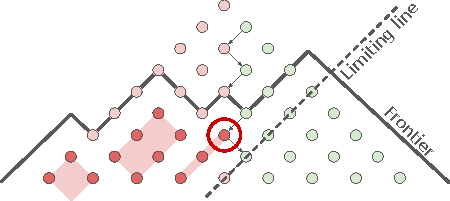
\includegraphics[width=0.85\linewidth]{images/dphpc-dynamic-priority-diagram.pdf}
  \caption{Visualization of the internal state of the dynamic priority algorithm. The circles are cells in the DP table (colored by worker). There are two workers (red and green). The state is from the perspective of the red worker. The arrows represent (past or future) sends and receives. Every cell on or above the \emph{frontier} is known to have been calculated by some worker. Every cell on or below the \emph{limiting line} cannot be calculated by the red worker at the moment.}
  \label{priority_state}
\end{figure}

In order to perform calculations whenever possible, it is necessary to determine which calculations are possible in a given state. Figure \ref{priority_state} shows the internal state that our algorithm keeps for this purpose. Every cell on the solid jagged line (\emph{frontier}) has been calculated by some worker, and every cell on or below the dotted line (\emph{limiting line}) can not be calculated at the moment. This means that all cells below the frontier and above the limiting line can be calculated without receiving any further messages from other workers. The frontier and the limiting lines fully determine the currently possible calculations (darker red).

The shape of the frontier is a direct consequence of the dependencies in our DP table. Before a DP cell can be calculated, the cells above it (left and right) must be calculated (see arrows in figure \ref{dp_table}). Because of transitivity, this means that all DP cells in the ``upside down pyramid'' ending in a cell must have been calculated before it. The frontier is the boundary of a union of such pyramids. Whenever a worker learns that a cell was calculated (because it calculated the value itself or received it from another worker) it extends its frontier by union with the pyramid ending in that cell.

Every worker has up to 2 limiting lines at any given time. These diagonal lines go through the next cell that the worker expects to receive. The worker shouldn't calculate any cells on or below a limiting line, since these cells will either be calculated by another worker (e.g. the cell that it expects to receive) or depend on values in such cells.

Once it is clear which cells are possible to calculate, it is necessary to choose a calculation order. One interesting case is outlined with a red circle in figure \ref{priority_state}. This cell has not been calculated yet, and another worker expects to receive its value. To prevent other workers from being blocked, such cells (and their dependencies) will be calculated before cells that do not result in a send. If there are no such cells to prioritize, cells near the middle of the DP pyramid are calculated first, since this order results in a frontier with few bends, which makes planning calculations faster.

\mypar{SIMD Optimization}
The amount of work needed per DP cell dynamically depends on the input, since the number of loop iterations in the while-loop is determined by the number of equal elements after a change. Therefore, the workload per worker might be imbalanced. %, especially for inputs with high similarity. 
To mitigate these imbalances and hence, reduce the time workers are waiting, we use x86's SIMD\footnote{``Single instruction stream, multiple data streams'' by Flynn's Taxonomy \cite{flynns_taxonomy}} vector extensions to compare multiple elements at once.

In many cases we need to compare only one value, because the first value is already unequal. In these cases we would not benefit from using SIMD instructions, they might even be more expensive. Therefore, we have a preliminary scalar check for inequality of the first element. Only if this check fails, we will use SIMD instructions.

%To force the compiler to use SIMD instructions we use the vector intrinsics from the \texttt{immintrin.h} %TODO: ref needed?) -> Intel intrinsics guide as footnote?
%header.
%If there are at least eight elements left in both input sequences, we will use the AVX\footnote{Advanced Vector Extensions and} instructions which operate on 8-way vectors of 32-bit integers. For the case, in which less than eight elements but at least four are left, we make use of SSE\footnote{Streaming SIMD Extensions are extensions to the x86 instruction set architecture} instructions once to compare 4-way vectors.

For the vectorized comparison we first load unaligned 8-way or 4-way vectors from both input sequences (the loads need to be unaligned, since we do not know the position in the vector in advance and we compare the input sequences at different offsets). Then we use a \texttt{cmpeq} intrinsic to compare the two vectors for equality. The result is then checked for an unequal element by using the negation of the \texttt{testc} intrinsic. If there is no inequality, the next vector will be checked. Otherwise, the exact location of the inequality is determined by a scalar loop over the last up to eight elements using the same loop as in the original algorithm.

\section{Experimental Results}\label{sec:exp}

%Here you evaluate your work using experiments. 
%You start again with a very short summary of the section.
%The typical structure follows.
In this section we first describe the experimental setup for our benchmarks, including the hardware and software used, the test cases and how we performed our measurements. Then we present our results where we compare to an existing implementation and evaluate the scaling of our implementations.

\mypar{Hardware \& software setup} % WARNING This name is referenced by hand below. Remember to change that too.
%Specify the platform (processor, frequency, maybe OS, maybe cache sizes)
%as well as the compiler, version, and flags used. If your work is about performance, 
%I strongly recommend that you play with optimization flags and consider also icc for additional potential speedup.
To evaluate our code with an increasing number of processing units, we ran our benchmarks on ETH's Euler cluster\footnote{For more information see \url{https://scicomp.ethz.ch/wiki/Euler}}. We used their 6th generation compute nodes with two 64-core AMD EPYC 7742 processors, which belongs to AMD's Zen 2 generation. The nodes are interconnected via a dedicated 100 Gb/s InfiniBand HDR network.

We compiled our C++ code locally using GCC 9.3.0 and Open MPI 4.0.3 with the flags \texttt{-std=c++17 -O3\linebreak -ffast-math \linebreak[1]-march=znver2}. For comparison with an existing implementation we use GNU diff utilites (diffutils) \cite{diffutils}. To have a fair comparison and to inject timers we recompiled it using their configure script with \texttt{CFLAGS=\linebreak[4]"-O3 -march=znver2 -ffast-math"} and then ran \texttt{make}. The diffutils binary is always called with the argument \texttt{--minimal} to avoid heuristics that do not necessarily produce the smallest edit distance. Our algorithms include SIMD features which can be enabled by preprocessor macros. Unless stated otherwise, these are enabled.

On Euler we load the modules \texttt{openmpi/4.0.2} and \texttt{python/3.6.4}. We then use separate jobs for different processor counts and submit them to the %IBM LSF (Load Sharing Facility)
batch system. For the job submission we use the resource requirement flag \texttt{-R \textquotesingle select[\linebreak[0]model\linebreak[0]==\linebreak[1]EPYC\_\linebreak[0]7742]\textquotesingle} to get the Euler VI nodes, \texttt{-R \textquotesingle rusage\linebreak[0][mem=512]\textquotesingle} to specify our memory usage of at most 512 MB per core and \texttt{-R \textquotesingle span[\linebreak[0]ptile\linebreak[0]=128]\textquotesingle} to ensure that we always use full nodes. For exclusive use of the nodes we request more cores if necessary to reach a multiple of 128.

%Then explain what kind of benchmarks you ran. The idea is to give enough information so the experiments are reproducible by somebody else on his or her code.
%For sorting you would talk about the input sizes. For a tool that performs NUMA optimization, you would specify the programs you ran.

\mypar{Test cases}
For testing and benchmarking we built a script to generate random test cases. Each test case consists of two input files containing one integer per line, representing the two input sequences to compute the longest common subsequence length for. For our benchmarks we generate two completely independent files (of equal length) using a Zipf distribution \cite{Zipf} where the probability for an integer value $v \in \left[0,\linebreak[0]\text{sequence\linebreak[2] length}\right)$ is proportional to $\frac{1}{v+1}$. We chose this distribution instead of an uniform distribution, because it models the fact that some tokens might be more frequent than others in texts written by humans.

We also used DNA nucleotide sequences for benchmarking, to check that our algorithms perform similarly as with synthetic inputs. We used two pairs of DNA which we obtained from GenBank \cite{genbank}, a shorter pair (streptomyces aureoverticillatus, {\raise.17ex\hbox{$\scriptstyle\mathtt{\sim}$}}171'000 base pairs, edit distance {\raise.17ex\hbox{$\scriptstyle\mathtt{\sim}$}}99'000) \cite{smallDNA1Data, smallDNA2Data} and a longer pair (synechococcus elongatus, {\raise.17ex\hbox{$\scriptstyle\mathtt{\sim}$}}\seqsplit{2'700'000} base pairs, edit distance {\raise.17ex\hbox{$\scriptstyle\mathtt{\sim}$}}1'800'000) \cite{bigDNA1Data, bigDNA2Data}.
%The generation process either generates two completely \emph{independent} files using a Zipf distribution or it generates only one random file and then random changes to it for the second file. 

%For the random changes we have test cases with only additions, only deletions (remove) or both. Also we can influence the selection of changed lines with two parameters. The change strength determines the percentage of edited lines relative to the lines in the first file. The chunkiness determines how contiguous the changed lines will be. Low chunkiness means many small independent changes, high chunkiness leads to large blocks of changes.

\mypar{Benchmarking methodology}
The programs are called repeatedly on each test case from a Python script. The measurements are repeated until the confidence interval, which contains the true \emph{median} with a probability of 95\%, has a relative error of at most 5\% around the current median estimate for the runtime, or a maximum of 50 repetitions is reached.

Each execution of a test case was limited to 120 seconds. If a combination of algorithm, parallelism and input size reached this time limit in any repetition, all repetitions for this combination were excluded from our results. This was done to avoid testing large inputs with low parallelism, which takes prohibitively long.

% runtime measurement
The runtime is measured using the \texttt{high\_\linebreak[0]resolution\linebreak[0]\_clock} from the \texttt{chrono.h} header. We measure this wall-clock time only on the dedicated MPI process which reads the input and prints the output. To measure time in diffutils we inserted calls to the \texttt{gettimeofday} function from \texttt{time.h} in \texttt{analyze.c}. In our benchmarks we focus on the computation time of the core algorithms, excluding the time needed for reading the input and writing output and also any precomputation done in diffutils. The runtimes are printed in microseconds.
%In the end the Pyhton script reads the runtimes in microseconds from the standard output using the \texttt{subprocess} module with pipes.

\mypar{Results}
Each marker in all following plots represents the calculation time for a single repetition. We calculate the median value across repetitions and connect these using linear interpolation to show trends.

We first investigate the performance of our parallel algorithms when limited to a single process. Figure \ref{results_sequential_comparison} shows the calculation time of our algorithms and diffutils. Our purely sequential baseline is faster than diffutils. This is expected: our comparison is not fair, since diffutils is calculating (but not outputting within the measured time) an edit script, whereas our algorithm only calculates the edit distance. Diffutils uses the recursive ``linear space refinement'' algorithm from \cite{myers_anond_1986} to calculate the edit script, which is ``roughly twice as slow as the basic $O(nd)$ algorithm'' \cite{myers_anond_1986} used in our baseline. Diffutils is not twice as slow as our sequential baseline - this is likely because diffutils has been well optimized over time. The MPI row-wise algorithm is faster than our sequential baseline. It is not clear why this is the case, since the core algorithm and compiler settings are identical, but the complete code for the MPI row-wise algorithm is more complex. The MPI dynamic priority algorithm seems clearly faster than all the others. This is due to the order in which it calculates the cells of the DP table. The algorithm prioritizes cells in the middle of the DP table (see \ref{sec:yourmethod}). This makes MPI dynamic priority faster, unless there are very different amounts of additions vs deletions, in which case it would be slower than the other algorithms.

\begin{figure}[hbt]\centering
  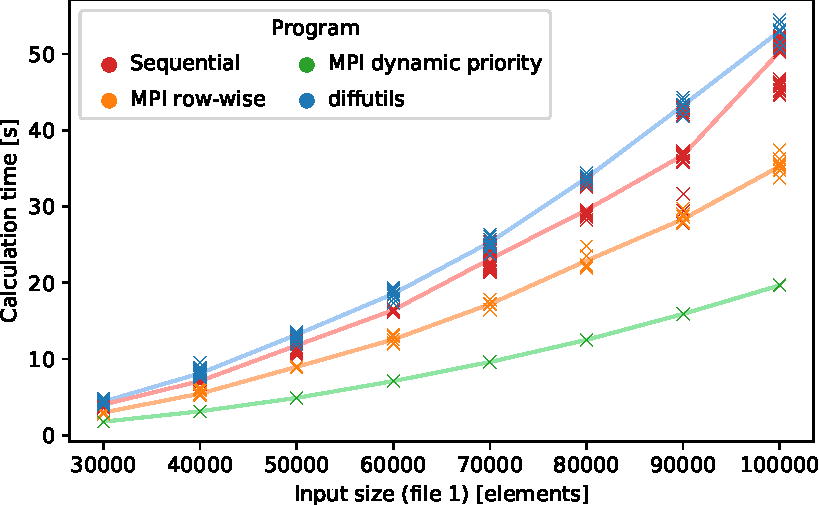
\includegraphics[width=\linewidth]{images/sequential-comparison.pdf}
  \caption{Calculation time of all algorithms when limited to a single process.}
  \label{results_sequential_comparison}
\end{figure}

To understand how our parallel algorithms scale, we ran them using various numbers of compute nodes. Figure \ref{results_scaling_time_mpi_row_wise} shows the calculation times from these experiments for our MPI row-wise algorithm. Using more nodes leads to a significant performance improvement. The curves for runtime seem to have approximately the ideal shape (proportional to $1 / \text{nodes}$). However it is not clear from this plot exactly how much less efficient the computation becomes as more nodes are used - that is investigated in a later plot. The runtime with DNA inputs shows the same trend as with synthetic inputs. For similar input sizes, the calculation time for DNA inputs is lower than for synthetic data, since they have a smaller edit distance.
% Unfortunately, the computing cluster was not available to run the large DNA input on all nodes, but we expect it to follow the same trend as the small DNA.

\begin{figure}[hbt]\centering
  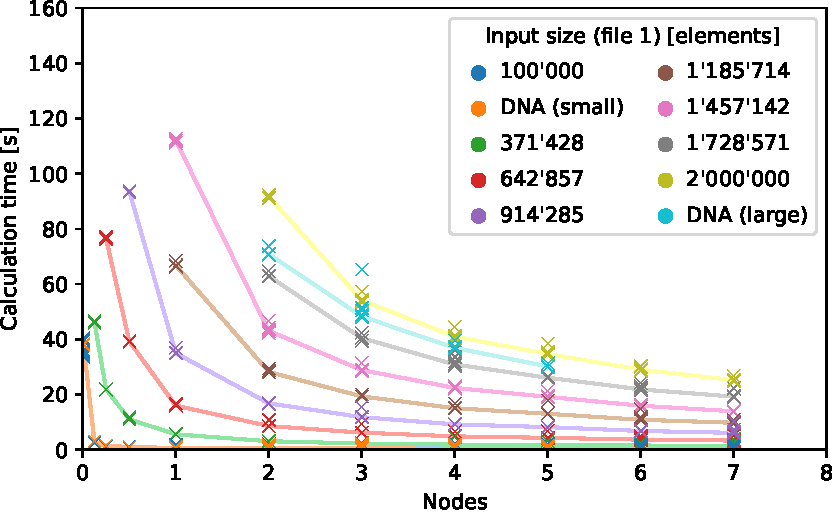
\includegraphics[width=\linewidth]{images/scaling-time-mpi-row-wise.pdf}
  \caption{Calculation time of the MPI row-wise algorithm with varying parallelism and input sizes.}
  \label{results_scaling_time_mpi_row_wise}
\end{figure}

Figure \ref{results_scaling_time_mpi_dynamic_priority} shows the results of an identical scaling experiment for our MPI dynamic priority algorithm. With one process the MPI dynamic priority algorithm is faster than MPI row-wise (as in figure \ref{results_sequential_comparison}). With half a node both algorithms have approximately the same speed. However the MPI dynamic priority algorithm becomes slower than the MPI row-wise algorithm once more nodes are used. This is surprising since the dynamic priority algorithm was designed to avoid blocking waits. We were not able to identify the cause of this bad scaling (which is difficult, since the behavior of the algorithm is very dynamic). Note that even with this inefficiency, using more nodes (for the number of nodes we tested) still reduces the total execution time. 

\begin{figure}[hbt]\centering
  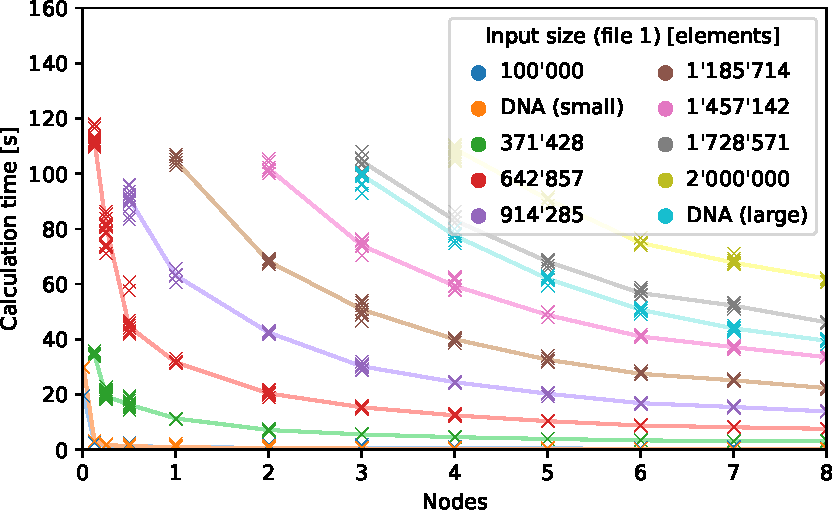
\includegraphics[width=\linewidth]{images/scaling-time-mpi-dynamic-priority.pdf}
  \caption{Calculation time of the MPI dynamic priority algorithm with varying parallelism and input sizes.}
  \label{results_scaling_time_mpi_dynamic_priority}
\end{figure}

To understand how efficiently our algorithms scale, we investigated the execution rate with a varying number of nodes (figure \ref{results_scaling_rate_mpi_row_wise}). We calculate rate as $\frac{n \cdot d}{t}$ which is the calculation time $t$ in seconds divided by the asymptotic runtime. For a fixed input (each curve in the plot), the rate is proportional to the speedup \cite{moreland2015formal} (which we do not calculate, since we do not have sequential measurements for large inputs). The dotted reference line approximates the rate that would be achieved with ideal linear speedup. This line is calculated based on the single run which achieves the highest rate with 1 node (for any input size). For the smallest input size (30'000 elements), the rate does not increase with more nodes. The overhead (e.g. MPI communication) likely dominates, since the total execution time (figure \ref{results_scaling_time_mpi_row_wise}) is very low. As inputs become larger, the row-wise algorithm becomes efficient. With the largest input sizes and number of nodes we tested, it scales nearly ideally.

\begin{figure}[hbt]\centering
  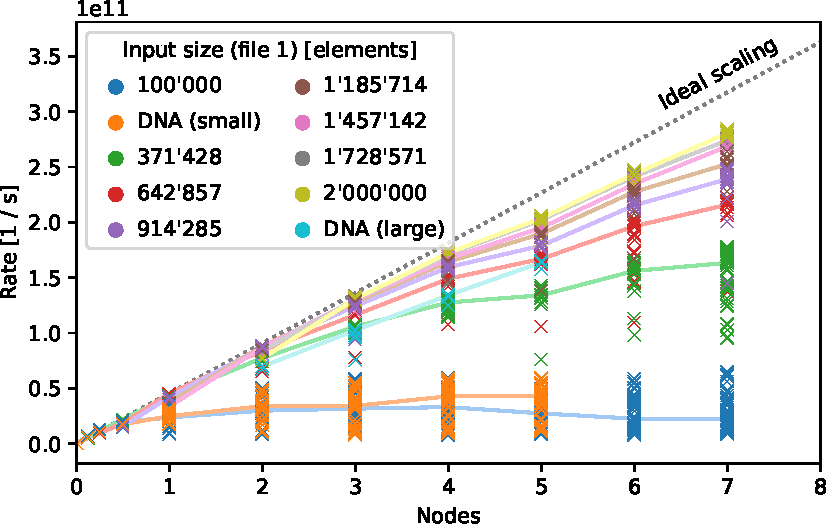
\includegraphics[width=\linewidth]{images/scaling-rate-mpi-row-wise.pdf}
  \caption{Rate of calculation (inverse runtime scaled by amount of work) of the MPI row-wise algorithm with varying parallelism and input sizes}
  \label{results_scaling_rate_mpi_row_wise}
\end{figure}

Figure \ref{results_scaling_rate_mpi_dynamic_priority} shows results in an identical format, but for our MPI dynamic priority algorithm. The MPI dynamic priority algorithm shows significantly worse than ideal scaling. Although the plotted curves for rate vs input size are roughly straight lines, the rate is not proportional to the number of nodes, as it would be for ideal scaling.

\begin{figure}[hbt]\centering
  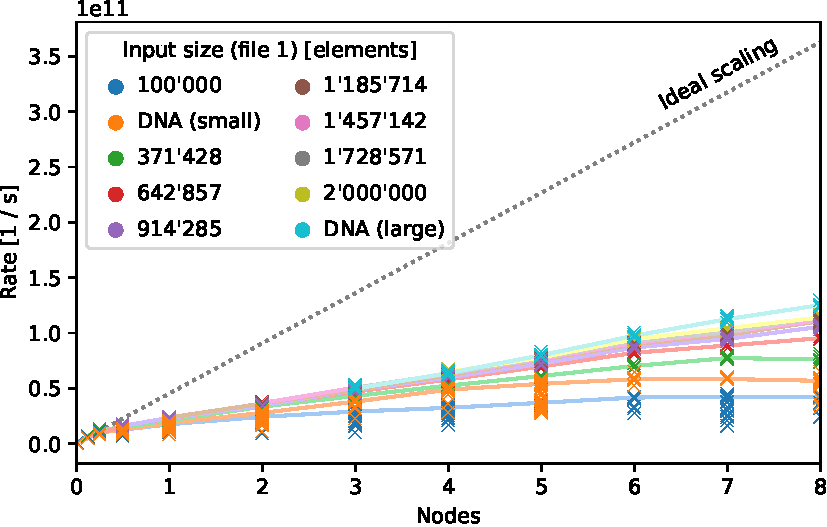
\includegraphics[width=\linewidth]{images/scaling-rate-mpi-dynamic-priority.pdf}
  \caption{Rate of calculation (inverse runtime scaled by amount of work) of the MPI dynamic priority algorithm with varying parallelism and input sizes}
  \label{results_scaling_rate_mpi_dynamic_priority}
\end{figure}

In all previously presented results, our algorithms had their SIMD features enabled (see ``Hardware \& software setup''). To investigate how this affects our algorithms, we repeated all the benchmarks from figures \ref{results_scaling_time_mpi_row_wise} and \ref{results_scaling_time_mpi_dynamic_priority} with the SIMD features disabled. Figure \ref{results_simd_comparison} shows the speedup from SIMD across those benchmarks. The speedup for each plotted point is calculated from the median runtime of each combination of algorithm, node count and input size. For the MPI row-wise algorithm, SIMD typically gives a speedup of 10\% - 30\%. Surprisingly enabling (the same) SIMD features in the MPI dynamic priority algorithm makes it run around 10\% slower. It is not clear what causes this slowdown. It may be necessary to investigate this together with the general scaling issues of the dynamic priority algorithm.

\begin{figure}[hbt]\centering
  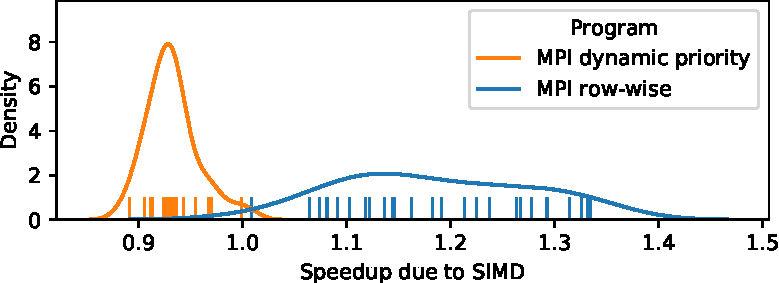
\includegraphics[width=\linewidth]{images/simd-comparison.pdf}
  \caption{Speedup (non-SIMD runtime / SIMD runtime) across all input sizes and node counts}
  \label{results_simd_comparison}
\end{figure}

% Next divide the experiments into classes, one paragraph for each. In each class of experiments you typically pursue one questions that then is answered by a suitable plot or plots. For example, first you may want to investigate the performance behavior with changing input size, then how your code compares to external benchmarks.
% 
% For some tips on benchmarking including how to create a decent viewgraph see pages 22--27 in Pueschel:10.

% {\bf Comments:}
% \begin{itemize}
% \item Create very readable, attractive plots (do 1 column, not 2 column plots
% for this report) with readable font size. However, the font size should also not be too large; typically it is smaller than the text font size.
% An example is in Fig.~\ref{fftperf} (of course you can have a different style).
% \item Every plot answers a question. You state this question and extract the
% answer from the plot in its discussion.
% \item Every plot should be referenced and discussed.
% \end{itemize}
% 
% \begin{figure}\centering
%   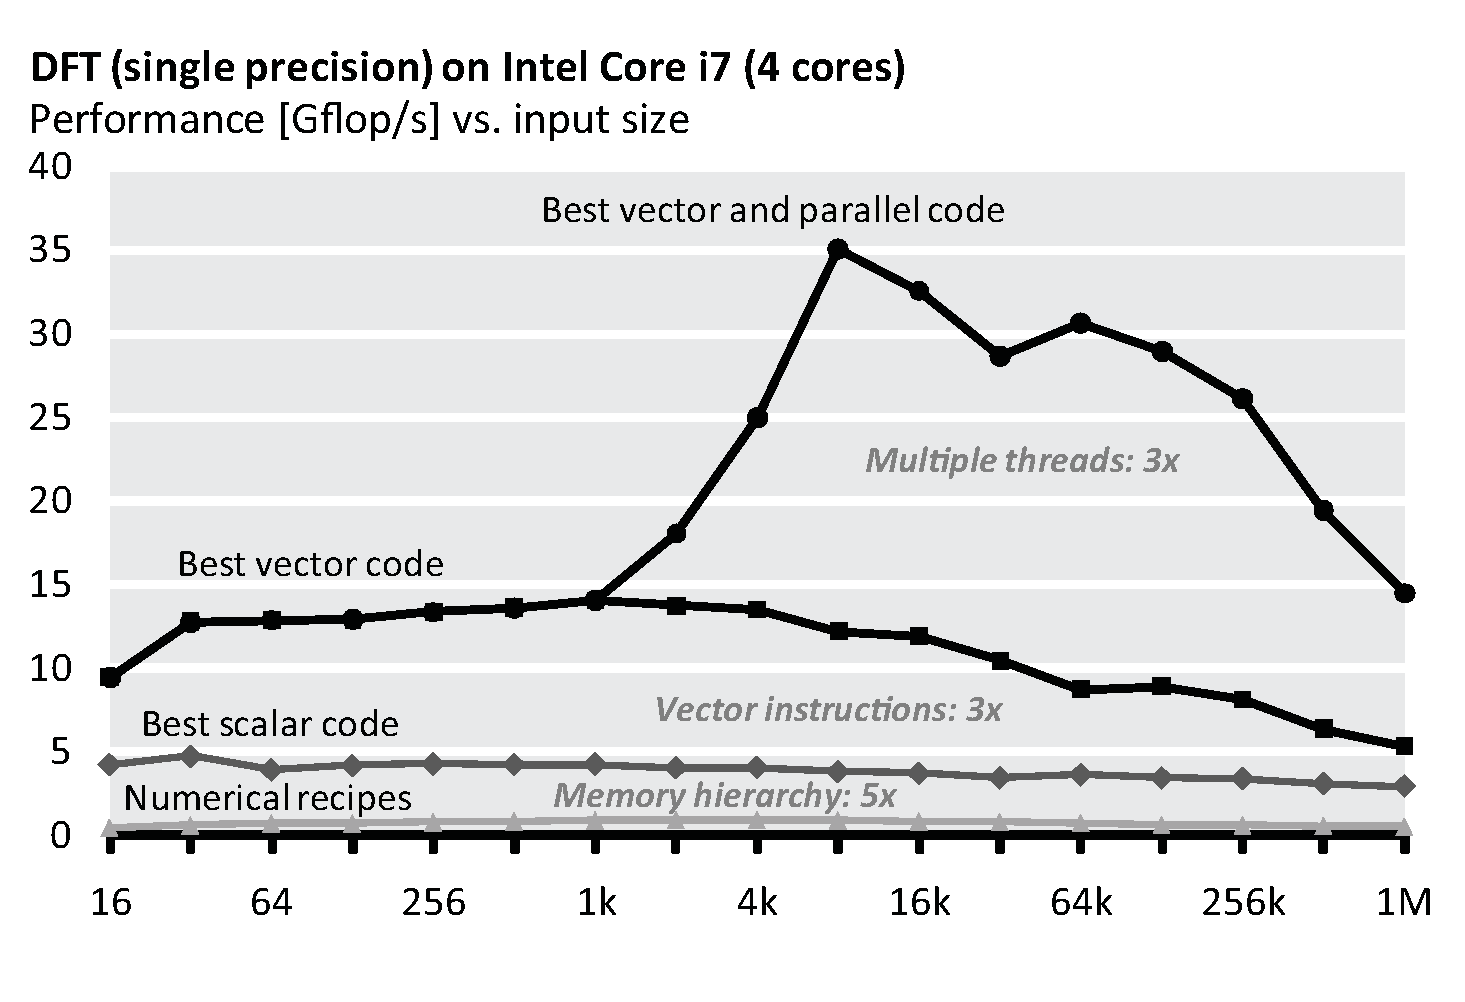
\includegraphics[scale=0.33]{dft-performance.eps}
%   \caption{Performance of four single precision implementations of the
%   discrete Fourier transform. The operations count is roughly the
%   same. The labels in this plot are maybe a little bit too small.\label{fftperf}}
% \end{figure}

\section{Conclusion}
In this report we presented a way to parallelize Myers' longest common subsequence algorithm and applied various optimizations. Our results showed that that our simple row-wise algorithm scales well to many processes. Our algorithms hold up against diffutils when run sequentially. Against our expectations, our dynamic priority algorithm does not scale well.

\mypar{Future work} 
In our work on this algorithm we considered various ideas to increase performance or reduce memory consumption, which we unfortunately did not have the time to experiment with for our report.

As such, we currently do not read out the edit script due to the quadratic memory consumption that it requires with this algorithm. If our algorithm is adapted to use Myers' recursive approach for linear space refinement \cite{myers_anond_1986} (which calls the non-recursive algorithm), it could output the edit script with only a minor performance cost.

It is possible that using SIMD to calculate multiple cells in parallel would improve the performance further.
    
% Here you need to summarize what you did and why this is
% important. {\em Do not take the abstract} and put it in the past
% tense. Remember, now the reader has (hopefully) read the report, so it
% is a very different situation from the abstract. Try to highlight
% important results and say the things you really want to get across
% such as high-level statements (e.g., we believe that .... is the right
% approach to .... Even though we only considered x, the
% .... technique should be applicable ....) You can also formulate next
% steps if you want. Be brief. After the conclusions there are only the references.

% \section{Further comments}

% Here we provide some further tips.

% \mypar{Further general guidelines}

% \begin{itemize}
% \item For short papers, to save space, I use paragraph titles instead of
% subsections, as shown in the introduction.
% 
% \item It is generally a good idea to break sections into such smaller
% units for readability and since it helps you to (visually) structure the story.
% 
% \item The above section titles should be adapted to more precisely
% reflect what you do.
% 
% \item Each section should be started with a very
% short summary of what the reader can expect in this section. Nothing
% more awkward as when the story starts and one does not know what the
% direction is or the goal.
% 
% \item Make sure you define every acronym you use, no matter how
% convinced you are the reader knows it.
% 
% \item Always spell-check before you submit (to us in this case).
% 
% \item Be picky. When writing a paper you should always strive for very
% high quality. Many people may read it and the quality makes a big difference.
% In this class, the quality is part of the grade.
% 
% \item Conversion to pdf (latex users only): 
% 
% dvips -o conference.ps -t letter -Ppdf -G0 conference.dvi
% 
% and then
% 
% ps2pdf conference.ps
% \end{itemize}
% 
% \mypar{Graphics} For plots that are not images {\em never} generate the bitmap formats
% jpeg, gif, bmp, tif. Use eps, which means encapsulate postscript. It is
% scalable since it is a vector graphic description of your graph. E.g.,
% from Matlab, you can export to eps.
% The format pdf is also fine for plots (you need pdflatex then), but only if the plot was never before in the format 
% jpeg, gif, bmp, tif.

% References should be produced using the bibtex program from suitable
% BiBTeX files (here: bibl_conf). The IEEEbib.bst bibliography
% style file from IEEE produces unsorted bibliography list.
% -------------------------------------------------------------------------
\bibliographystyle{IEEEbib}
\bibliography{bibl_conf}

\end{document}
